\chapter[\hspace{0pt}基于多扫描Mamba的高分辨率病理图像分类研究]{{\heiti\zihao{3}\hspace{0pt}基于多扫描Mamba的高分辨率病理图像分类研究}}\label{chapter3: 基于多扫描Mamba的高分辨率病理图像分类研究}
\removelofgap
\removelotgap
本章研究了基于多扫描Mamba的高分辨率病理图像分类研究,通过整合多种扫描模式分支的特征信息,引入病理图像的空间信息,提高Mamba建模2D空间关系的能力,进而提高高分辨率病理图像分类性能。
本章内容共分为四节,\hyperref[section3: 研究动机]{第一节}介绍研究的动机;\hyperref[section3: 问题描述和符号定义]{第二节}介绍问题的描述与符号定义;
\hyperref[section3: 基于空间信息增强的多扫描Mamba模型]{第三节}介绍本章提出的基于空间信息增强的多扫描Mamba模型;
\hyperref[section3: 实验设置及结果分析]{第四节}给出实验设置和结果分析;\hyperref[section3: 本章小结]{第五节}对本章进行总结与讨论。

\section[\hspace{-2pt}研究动机]{{\heiti\zihao{-3} \hspace{-8pt}研究动机}}\label{section3: 研究动机}

%\subsection[\hspace{-2pt}研究动机]{{\heiti\zihao{4} \hspace{-8pt}研究动机}}\label{section3: 研究动机}

病理图像的多实例学习范式中,由于病理图像的分辨率过高,往往面临实例数量庞大、信息繁杂等问题,因此如何高效地提取实例关系并突出关键实例特征一直是多实例学习的核心。
近年来,Mamba模型凭借其高效的计算速度和强大的数据建模能力,逐渐被引入病理图像多实例学习领域,并在特征聚合方面取得了瞩目的效果。
然而,Mamba模型本质是一类序列学习方法,其输入是单个序列,而单个序列无法体现出视觉的空间关系,
因而单个序列扫描模式的Mamba模型的性能会受其空间关系建模的限制。

为了缓解上述所提到的问题,业内主流的解决方案是将多个扫描模式序列的信息进行整合。
然而,如~\ref{figure3: 扫描示意图}左图所示,大多数方法虽然通过类似横向和竖向的扫描模式缓解了Mamba序列敏感特性和视觉任务的差异,但是依旧只是在一维序列中进行,并没有充分利用视觉任务的特性如局部连续性、旋转不变性等,
更没有关注到空间信息的捕获。为此,本章从引入局部连续性、旋转不变性的视觉特性出发,提供了两种新的扫描模式,综合多个扫描模式分支以建模出更全面特征。
此外,本章还通过进一步综合局部空间信息,来提高模型对视觉任务的适配。

\begin{figure}[h]
  \centering
  \captionsetup{font={small, stretch=1.312}}
  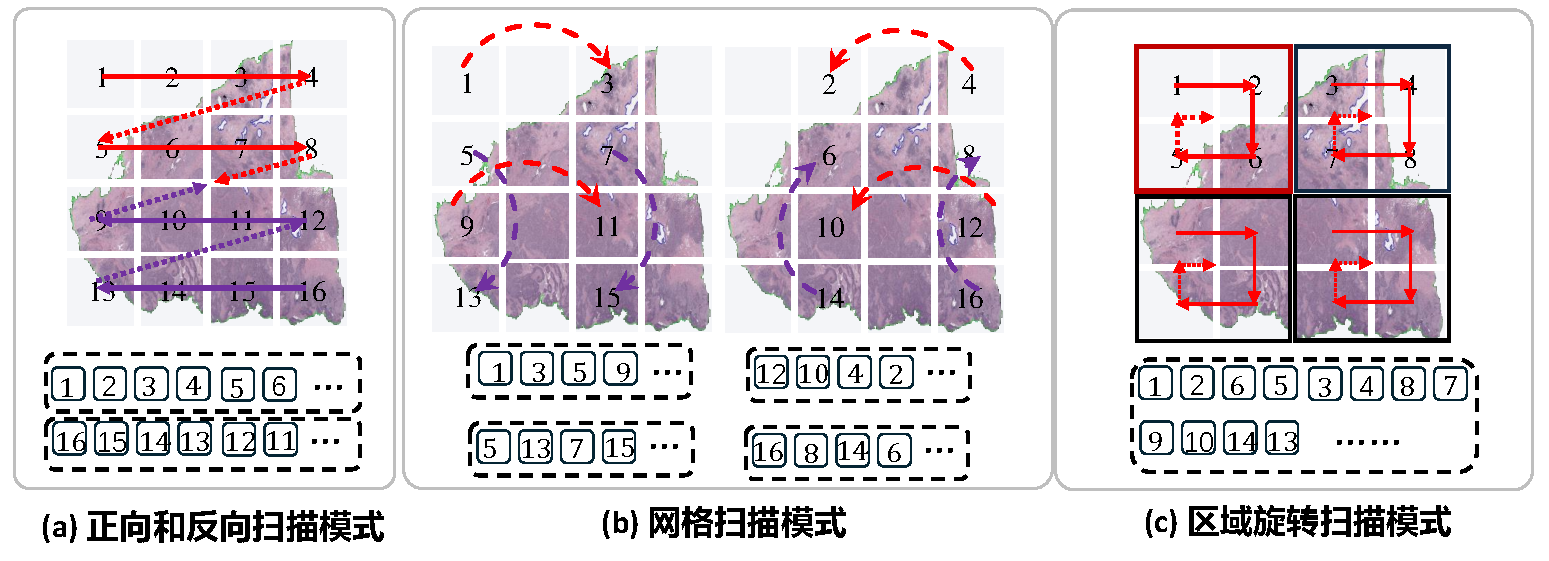
\includegraphics[width=\columnwidth]{figures/多扫描模式.pdf}
  % \captionsetup{justification=justified,singlelinecheck=false}
  \bicaption[常规扫描、网格扫描和区域螺旋扫描示意图]{常规扫描、网格扫描和区域螺旋扫描示意图。}[Schematic diagram of conventional scan, grid scan and region spiral scan]{Schematic diagram of conventional scan, grid scan and region spiral scan.}
  \vspace{-10pt}
  \label{figure3: 扫描示意图}
  \end{figure}

\section[\hspace{-2pt}问题描述和符号定义]{{\heiti\zihao{-3} \hspace{-8pt}问题描述和符号定义}}\label{section3: 问题描述和符号定义}

本研究采用多实例学习范式构建高分辨率病理图像分类模型,其数据集由 WSI 全切片图像与对应标签构成的样本对$(X,Y)$组成,
\begin{equation}
  D=\{(X_1,Y_1),...,(X_j,Y_j),...,(X_n,Y_n)\},
\end{equation}
其中,$n$为数据集样本数量。
每一个WSI切片 $X_j$都被视为一个包,将其Patch视为该包中的实例,可以表示为 $X_j=\{x_i^j\}_{i=1}^N$。实例数量$N$因包而异。
包的类别由其中实例类别综合可得。如果一个包包含至少一个阳性实例,则认为它是阳性的;否则,它被归类为负包:

\begin{equation}
  Y(X)=\left \{
  \begin{array}{cl}
      0 &  if  \sum_{x \in X} y(x) = 0, \\
      1 & otherwise.
  \end{array}\right.
  \label{eq}
\end{equation}

在多实例学习范式中,样本包级标签$Y(X)$作为监督信号已知,而实例级标签$y(x)$则保持隐式状态。
该学习机制的核心目标在于通过聚合实例层特征信息,即用所有实例$\hat{Y}\gets\mathcal{M}\left(X\right)$预测包标签,最终实现病理图像的准确分类。
根据最近流行的方法,MIL预测过程可以分为三个步骤:实例特征提取、实例特征聚合和包分类。具体来说,这个过程可以定义如下:
\begin{equation}
  \hat{\mathnormal{Y}} \leftarrow \mathcal{M}(X):=\mathcal{C}(\mathcal{A}(\mathcal{F}(X))),
\label{eq1}
\end{equation}
其中$\mathcal{F}\left(\cdot\right)$、$\mathcal{A}\left(\cdot\right)$和$\mathcal{C}\left(\cdot\right)$分别是上述步骤的映射函数。

由于同一包中存在大量实例,因此WSI分类问题可以看作是一个长序列建模问题。基于现代状态空间模型(SSM),前人设计了结构化状态空间序列模型(S4)和Mamba等几种适合长序列建模的方法。经典的S4模型可以写成线性递归式:
\begin{equation}
  \begin{aligned}
    h_t&=\mathbf{\bar{A}}h_{t-1}+\mathbf{\bar{B}}x_{t},\\
    y_t&=\mathbf{C}h_t.
  \end{aligned}
  \label{eq32}
  \end{equation}
其中$\mathbf{\bar{A}}$表示离散化后的状态矩阵,$\mathbf{B}$和$\mathbf{C}$表示投影参数,$\mathbf{\bar{B}}$为离散化后的$\mathbf{B}$。另外,模型可以使用卷积模式计算输出:
\begin{equation}
  \begin{aligned}
      \bar{\mathbf{K}}&=(\mathbf{C\bar{B},C\bar{A}\bar{B}},\dots,\mathbf{C}\bar{\mathbf{A}}^{N-1}\bar{\mathbf{B}}),\\
      Y&=X*\bar{\mathbf{K}},
  \end{aligned}
  \label{eq33}
  \end{equation}
其中$K\in R^L$表示一个结构化卷积核,$N$表示输入序列$X$的长度。

Mamba进一步将选择机制集成到S4模型中,通过高效的硬件感知并行算法,使参数动态依赖于输入。
这允许Mamba根据当前上下文有选择地沿着序列传播或忘记信息,从而实现高效的长序列建模。
因此,结合Mamba的多实例学习范式可以被定义:
\begin{equation}
  \hat{Y} \leftarrow \mathcal{M}\left(X\right):=\mathcal{C}(\mathcal{A}(\Psi(\mathcal{F}(X)))),
\end{equation}
其中$\Psi\left(\cdot\right)$表示为Mamba模型。


\section[\hspace{-2pt}基于空间信息增强的多扫描Mamba模型]{{\heiti\zihao{-3} \hspace{-8pt}基于空间信息增强的多扫描Mamba模型}}\label{section3: 基于空间信息增强的多扫描Mamba模型}

\subsection[\hspace{-2pt}方法概述]{{\heiti\zihao{4} \hspace{-8pt}方法概述}}\label{section3: 方法概述}

\begin{figure}[h]
  \centering
  \captionsetup{font={small, stretch=1.312}}
  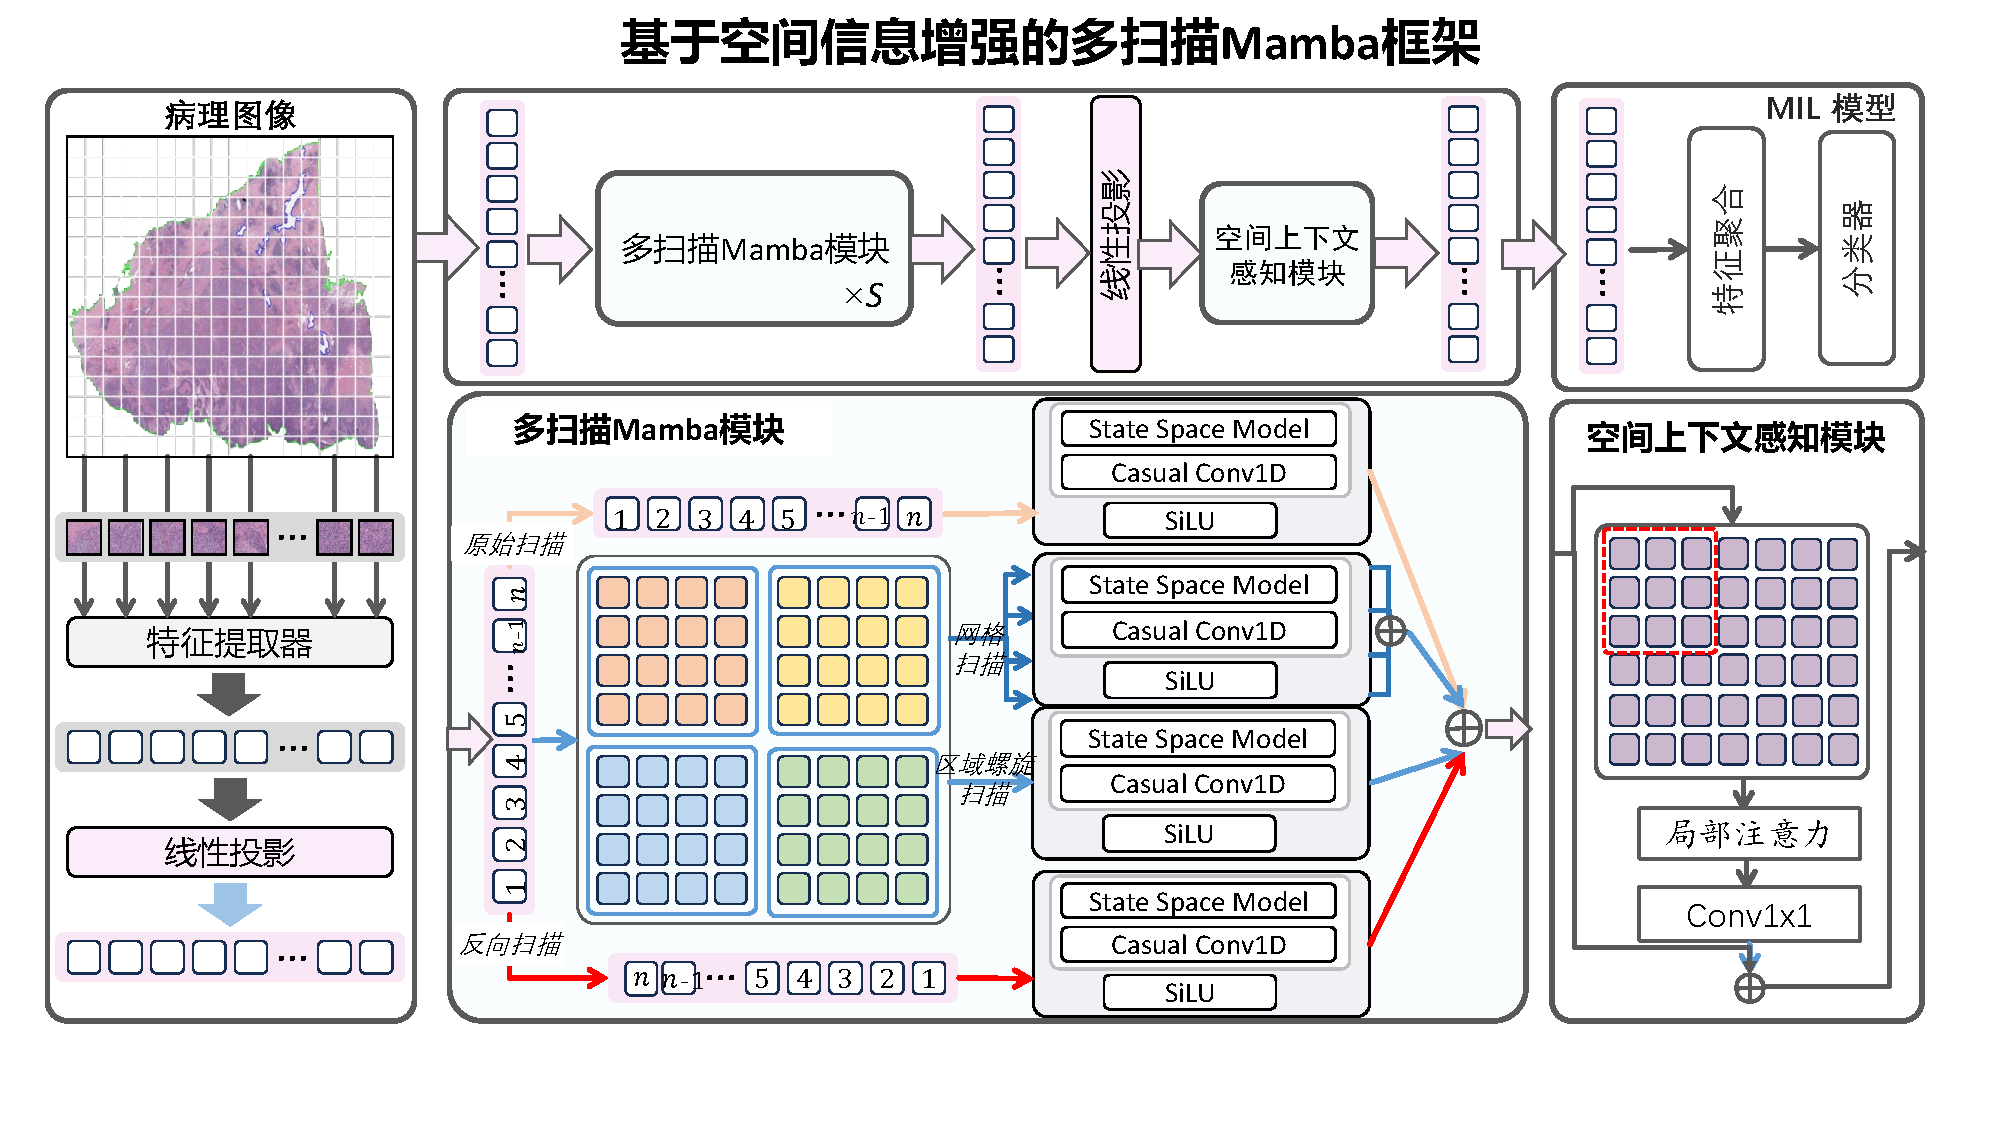
\includegraphics[width=\columnwidth]{figures/MMSMIL.pdf}
  % \captionsetup{justification=justified,singlelinecheck=false}
  \bicaption[基于多扫描Mamba的多实例学习架构示意图]{基于多扫描Mamba的多实例学习架构示意图。}[Illustration of the multi-instance learning architecture with multi-scan Mamba]{Illustration of the multi-instance learning architecture with multi-scan Mamba}
  \vspace{-10pt}
  \label{figure3: 多扫描Mamba}
  \end{figure}

为了解决~\ref{section3: 研究动机}小节中的问题,如图~\ref{figure3: 多扫描Mamba}所示,本章提出了一种名为基于空间信息增强的多扫描Mamba模型,该模型既发挥了Mamba长序列建模能力强的特点,同时也缓解其和视觉2D图像任务间的差异。
具体而言,本研究通过添加区域螺旋扫描和网格扫描等多种扫描模式分支,引入局部连续性、旋转不变性等的2D图像特性。
此外,为了进一步整合2D空间关系信息,本章引入一个2D空间上下文感知模块。总的来说,本研究的贡献如下:
\begin{itemize}
 \item 本研究提出了一种基于多扫描Mamba的多实例学习架构,命名为M$^2$S-MIL。M$^2$S-MIL通过添加区域螺旋扫描和网格扫描等扫描模式,引入2D图像的局部依赖和旋转不变性等,使之更适合病理图像分类任务。
 \item	针对视觉领域的2D属性,设计了新的扫描模式:区域螺旋扫描模式和网格扫描模式,引入了更多局部依赖、旋转不变性等2D空间信息,缓解顺序敏感的Mamba与病理图像分类任务间的差异。
 \item	为了进一步整合提升2D空间关系信息,本章设计了一个2D空间上下文感知模块,采用分块局部注意力,进一步融合局部相邻的实例信息,进一步提高模型性能。
\end{itemize}

\subsection[\hspace{-2pt}预处理与特征提取]{{\heiti\zihao{4} \hspace{-8pt}预处理与特征提取}}\label{section3: 预处理与特征提取}

给定一个WSI图片,参照CLAM~\cite{lu2021data}的设置,本章将之裁剪成一系列$256\times256$的非重叠图块,放大倍数为$20$倍,同时丢弃背景区域(饱和度$< 15$)。
本章采用ResNet-50~\cite{ROYERCARFAGNI2001253}或UNI~\cite{chen2024towards}作为底层特征提取器$\mathcal{F}\left(\cdot\right)$,对每个实例提取特征得到1024维的原始特征。
为了减少特征冗余和计算消耗,使用多层感知器(MLP)层将这些特征从1024减少到512。
数字病理图像的特征提取过程为:
\begin{equation}
  z_i= \mathcal{F}_\varphi(x_i) \in \mathbb{R} ^d.
\end{equation}
在该模型架构中,$\mathcal{F}_\varphi(\cdot)$被定义为骨干特征提取网络,其参数 $\varphi$表示特征学习模块的可训练参数集,通常其不与后续网络一起端到端训练,$d= 512$。
最后,一个WSI由一个连续长序列表示。
本章将之定义为原始扫描序列$Z_{origin}=\{z_i\}_{i=1}^N$,其中$z_i$是$X$的第$i$个实例的提取特征,$N$是实例的个数。

\subsection[\hspace{-2pt}多扫描Mamba模块]{{\heiti\zihao{4} \hspace{-8pt}多扫描Mamba模块}}\label{section3: 多扫描Mamba模块}

为了使Mamba能充分学习到实例间的相互依赖,并缓解其本身因果建模倾向所带来的负面影响,
本章方法提出使用多种扫描模式,以消除单一扫描序列所建模出的偏执,捕获实例间更全面的特征信息。
如图~\ref{figure3: 多扫描Mamba}所示,在多扫描Mamba模块中可分为四个扫描分支:原始扫描序列分支、反向扫描序列分支、区域螺旋扫描分支和网格扫描分支。
首先,原始扫描模式序列被输入Mamba模型以提供常规特征:
\begin{equation}
  Z'_{origin}=\Psi_{origin} (Z_{origin}),
\end{equation}
其中,$\Psi_{origin}(\cdot)$同~\ref{section3: 问题描述和符号定义}小节所示为Mamba模型。 反向扫描序列以初步缓解Mamba不过分学习到正向序列的特有顺序偏执:
\begin{equation}
  Z'_{flip}=\Psi_{flip} (Z_{flip})=\Psi_{flip} (\{z_i\}_{i=N}^1).
\end{equation}
为进一步引入空间信息,本章精心设计了两种新的扫描模式:区域螺旋扫描和网格扫描模式。
其中,区域螺旋扫描被设计以引入局部连续性和旋转不变性等2D图像属性,网格扫描模式用于在一个序列中捕获多个方向上的信息。




具体而言,输入的实例特征序列首先被重塑为2D特征图,初始的二维特征图形式为$H\in \mathbb{R} ^{N\times D}$,
之后转变为$ H \in \mathbb{R} ^{\lceil\sqrt{N}\rceil \times \lceil\sqrt{N}\rceil \times D}$。
重塑后便可如图~\ref{figure3: 扫描示意图}所示的网格扫描方式。网格子序列1可表示为:
\begin{equation}
  %Z_{grid1}=\{z_{ij},i=2k+1,k<=\lfloor \lceil\sqrt{N}\rceil/2\rfloor , k \in \mathbb{N}_0;j=2m+1,m<=\lfloor \lceil\sqrt{N}\rceil/2\rfloor,m \in \mathbb{N}_0.\}
  Z_{\text{grid1}} = \left\{ z_{ij} \,\big|\, 
i = 2k + 1,\, j = 2m + 1,\, 
k, m \in \mathbb{N}_0,\, 
k, m \leq \left\lfloor \frac{\lceil \sqrt{N} \rceil}{2} \right\rfloor 
\right\}.
\label{Z_grid1}
\end{equation}

同理,网格序列集合2、3、4可分别表示为:
\begin{equation}
  \begin{aligned}
  Z_{\text{grid2}} &= \left\{ z_{ij} \,\big|\, 
  i = 2k,\, j = 2m + 1,\, 
  k, m \in \mathbb{N}_0,\, 
  k, m \leq \left\lfloor \frac{\lceil \sqrt{N} \rceil}{2} \right\rfloor 
  \right\}, \\
  Z_{\text{grid3}} &= \left\{ z_{ij} \,\big|\, 
  i = 2k + 1,\, j = 2m + 1,\, 
  k, m \in \mathbb{N}_0,\, 
  k, m \leq \left\lfloor \frac{\lceil \sqrt{N} \rceil}{2} \right\rfloor 
  \right\}, \\
  Z_{\text{grid4}} &= \left\{ z_{ij} \,\big|\, 
  i = 2k,\, j = 2m,\, 
  k, m \in \mathbb{N}_0,\, 
  k, m \leq \left\lfloor \frac{\lceil \sqrt{N} \rceil}{2} \right\rfloor 
  \right\}.
  \end{aligned}
  \label{Z_grid234}
\end{equation}
网格扫描模式所得的四个子序列(都是原始特征集合的一部分)被分别输入Mamba后,将所输出子序列拼接在一起并还原回原本的位置。
\begin{equation}
  Z'_{grid}=Concat({\Psi^1_{grid} (Z_{grid1})},{\Psi^2_{grid} (Z_{grid2})},{\Psi^3_{grid} (Z_{grid3})},{\Psi^4_{grid} (Z_{grid4}))}.
\end{equation}
网格扫描模式在同一序列中综合多方向信息,以缓解单一扫描模式序列所带来的顺序偏向。

同时,如图~\ref{figure3: 扫描示意图}所示,特征图$H$被均匀划分为$L\times L$个非重叠式区域,以便于进行区域螺旋扫描。每个区域由 $M\times M$ 个实例构成,
并且满足关系:$L \times M=\left\lceil\sqrt{N}\right\rceil$。此外,为确保区域数量为$(L,L)$时能整除特征图大小,本章将对特征图进行零填充操作。
因此 特征图 $H$ 被划分为 ${\{H^l\}}^{L^2}_{l=1},H \in \mathbb{R} ^{M\times M\times D}$。
本章在划分后的区域内分别进行区域螺旋扫描,
得到序列$Z_{spiral}$($Z_{spiral}$由螺旋扫描唯一确定),并将螺旋扫描序列输入到Mamba进行建模,得到序列:
\begin{equation}
  Z'_{spiral}=\Psi_{spiral} (Z_{spiral}).
\end{equation}

该扫描模式相较于LocalMamba~\cite{huang2024localmamba}不仅引入了局部连续性,同时引入了2D病理图像的旋转不变性,进一步加强了空间信息,提高Mamba模型对视觉特性的建模能力。

最后,将四种扫描模式经由Mamba建模的实例序列分别还原至原始位置后,相互融合,
得出多扫描分支Mamba模块的输出序列:
\begin{equation}
  Z_{multi\_scan}=Merge(Z'_{origin}, Z'_{flip}, Z'_{grid}, Z'_{spiral}),
\end{equation}
其中$Merge(\cdot)$表示将四个分支序列对应融合成一个序列。本章将$Z_{multi\_scan}$作为多扫描Mamba模块的输出。除非特殊说明,本章中的多扫描Mamba模块层数$S$设为1。
综合了多种扫描模式的Mamba,不仅保留了Mamba本身极强的建模能力,并且还引入了二维空间信息、视觉特性等,更加适配病理图像分类任务。

\subsection[\hspace{-2pt}2D空间上下文感知模块]{{\heiti\zihao{4} \hspace{-8pt}2D空间上下文感知模块}}\label{section3: 2D空间上下文感知模块}

为了进一步提升模型捕获空间信息的能力,本章将综合多种扫描信息的序列特征输入到基于分块局部注意力的2D空间上下文感知模块中。
如图~\ref{figure3: 多扫描Mamba}所示,本章将输出的1D特征序列再次重塑为2D特征图($H'\in \mathbb{R} ^{\left\lceil\sqrt{N}\right\rceil\times\left\lceil\sqrt{N}\right\rceil\times D}$),
然后将特征划分为固定大小($M' \times M'$)的局部窗口(不同于上一小节的区域),每窗口内计算局部注意力。
并通过$1 \times 1$卷积还原原本的分辨率,避免信息损失。记某一个窗口内的输入特征为$H'_{win}$,则窗口内特征图可表示为:
\begin{equation}
\begin{aligned}
  Q_{\mathrm{win}}=\operatorname{Conv}_{1 \times 1}\left(H'_{\mathrm{win}}\right),
  &\quad K_{\mathrm{win}}=\operatorname{Conv}_{1 \times 1}\left(H'_{\mathrm{win}}\right),
  \quad V_{\mathrm{win}}=\operatorname{Conv}_{1 \times 1}\left(H'_{\mathrm{win}}\right),\\
  &H''_{win}=\operatorname{Conv}_{1 \times 1}\left(\sigma\left(\frac{Q_{\mathrm{win}} K_{\mathrm{win}}^{T}}{\sqrt{d_{k}}}\right) V_{\mathrm{win}}\right) ,
\end{aligned}
\end{equation}
其中$\sigma$是softmax函数,$Q_{\mathrm{win}}$, $K_{\mathrm{win}}$和$V_{\mathrm{win}}$分别是局部注意力机制的窗口内查询特征、窗口内键特征、窗口内值特征。
最后,全局的特征图$H'''$是通过分块局部注意力结果$H''$和多扫描分支Mamba模块的结果$H'$残差连接而得。
\begin{equation}
  \begin{aligned}
    H'''= H''+ H',
  \end{aligned}
  \end{equation}
因此,本章可以获得一个包含2D空间信息特征图$H'''\in \mathbb{R} ^{\left\lceil\sqrt{N}\right\rceil\times\left\lceil\sqrt{N}\right\rceil\times D}$,并将之转换为1D实例序列$Z_{output}=\{z^1_{output},z^2_{output},...,z^N_{output}\}$。


\subsection[\hspace{-2pt}基于Mamba的实例聚合]{{\heiti\zihao{4} \hspace{-8pt}基于Mamba的实例聚合}}\label{section3: 基于Mamba的实例聚合}

在特征融合阶段,本小节采用基于注意力机制的特征融合策略。
具体而言,构建包含双全连接层的上下文感知注意力模块,通过可训练参数动态计算每个实例特征的注意力权重。
该权重能够有效量化各实例特征对包级分类决策的贡献程度,进而通过加权平均操作将实例级特征整合为最终的包特征表示:
\begin{equation}
  \mathbf{b}=\mathcal{A}(Z_{output})=\sum_{i=1}^{N}a_iz^i_{output}.
\end{equation}
%其中,$a_i$表示第$i$个实例代表对应的可学习权重。
在该模块中,$a_i$被定义为第$i$个实例特征对应的可训练注意力权重参数。该参数通过反向传播机制动态优化,用于量化实例特征对包级分类决策的贡献程度,并满足归一化约束条件$\sum_{i=1}^{N}a_i = 1$:
\begin{equation}
  a_{i}=\frac{\exp\{u^{\mathrm{T}}\tan(v{z^i_{output}}^{\mathrm{T}})\}}{\sum_{j=1}^{N} \exp\{u^{\mathrm{T}}\tan(v{z^j_{output}}^{\mathrm{T}})\}}, 
\end{equation}
其中,$u$和$v$分别表示两个全连接层的网络参数。

\subsection[\hspace{-2pt}模型优化和推理]{{\heiti\zihao{4} \hspace{-8pt}模型优化和推理}}\label{section3: 模型优化和推理}

预测的包标签可以通过将包的表示输入分类器$\mathcal{C}\left(\cdot\right)$得到:
\begin{equation}
  \hat{Y}\gets\mathcal{C}\left(\mathbf{b}\right):= \mathcal{C}(\mathcal{A}(Z_{output})).
\end{equation}

本章内容仅使用常规的分类损失。包级分类预测的损失值通过交叉熵损失函数计算,其数学定义如式~\ref{loss1}所示:
\begin{equation}
  \mathcal{L}_{cls}=Y \log\hat{Y}+(1-Y)\log(1-\hat{Y}),
  \label{loss1}
\end{equation}
其中,$Y$表示包的真实标签,$\hat{Y}$则表示包预测标签。
综合上述内容,该模型的优化过程能够用如下公式来呈现,并且通过反向传播算法来求解得出整个模型的最优参数。

\begin{equation}
\{\hat{\Psi},\hat{\mathcal{R}},\hat{u},\hat{v},\hat{\mathcal{C}}\} \gets\arg{ \min_{\Psi,\mathcal{R},u,v,\mathcal{C}}{\mathcal{L}}}=\mathcal{L}_{cls},
\end{equation}
其中$\Psi$是本章所有Mamba架构的参数,$\mathcal{R}$表示本章空间上下文感知模块的参数,$u,v$分别表示基于注意力机制的聚合模块中两个全连接层的网络参数,$\mathcal{C}$为分类器的网络参数。

在推理阶段,本章采用和训练阶段保持一致的流程。同样采用四种扫描模式获取四个扫描序列分支分别输入Mamba架构,而后经过2D空间上下文感知模块进行空间结构信息增强,
最后采用基于注意力机制的聚合模块聚合包特征,并通过分类器进行推断分类。


\section[\hspace{-2pt}实验设置及结果分析]{{\heiti\zihao{-3} \hspace{-8pt}实验设置及结果分析}}\label{section3: 实验设置及结果分析}

在本节中,首先介绍了本章方法的实验设置,包括实验所用环境、数据集、评估指标和实施细节,
然后分析了基于多扫描Mamba的高分辨率病理图像分类实验结果,接下来对模型的各个模块以及超参数进行了消融实验和分析,最后对模型所关注的重点区域进行了可视化分析。

\subsection[\hspace{-2pt}实验设置]{{\heiti\zihao{4} \hspace{-8pt}实验设置}}\label{section3: 实验设置}

\textbf{(1)实验环境}

本章节的实验工作基于实验室高性能计算平台完成,该平台搭载AMD Ryzen 5700X 20 核中央处理器与 3 块 NVIDIA RTX 3090 图形处理器。
实验框架基于 Python 编程语言构建,采用 OpenSlide 库实现病理图像的高效读取,基于 Matplotlib 库完成数据可视化。详细的实验环境参数配置见表~\ref{table3: env}:

\begin{table}[h!]
  \small    % 设置表格字体为5号
  \setstretch{1.245}        % 设置具有指定弹力的橡皮长度(原行宽的1.2倍)
  \captionsetup{font={small, stretch=1.512}}
  \centering
  \bicaption[基于空间信息增强的多扫描Mamba模型的实验环境及配置]{基于空间信息增强的多扫描Mamba模型的实验环境及配置}[Experimental environment and configuration of M$^2$SMIL ]{Experimental environment and configuration of M$^2$SMIL}
  \begin{tabularx}{\textwidth}{CcCC}
  \toprule
  设备     & 配置               & 版本          & 数量 \\ 
  \midrule
  操作系统   & Ubuntu           & 20.04.4 LTS & 1  \\
  CPU    & AMD Ryzen 5700X  & -           & 1  \\
  GPU    & GeForce RTX 3090 & -           & 3  \\
  IDE    & VsCode           & 1.86.2      & 1  \\
  编程语言   & Python           & 3.10.11       & -  \\
  深度学习框架 & Pytorch          & 2.0.1       & -  \\
  \bottomrule
  \end{tabularx}
  \label{table3: env}
  \end{table}

\textbf{(2)数据集}

本章通过三个WSI分析子任务来评估M$^2$S-MIL模型:癌症诊断、亚型分类和生存预测。
对于癌症诊断任务,尽管已有大量研究~\cite{li2021dual,shao2021transmil,tang2023multiple} 基于 CAMELYON-16\cite{bejnordi2017diagnostic}数据集对不同模型在癌症诊断任务中的性能进行了评估,
但该数据集仅包含 400 张病理图像,数量上的局限性对模型评估的全面性与准确性造成了显著影响。
因此,为克服这一问题,本章参照文献\cite{lu2021data,tang2024feature}的做法,将 CAMELYON-16\cite{bejnordi2017diagnostic}数据集与 CAMELYON-17\cite{bandi2018detection} 数据集进行合并,
构建了一个包含 899 张病理图像的综合性 CAMELYON 数据集。这一策略在一定程度上缓解了数据量匮乏导致的评估困境,为模型性能评估提供了更为丰富和可靠的数据基础。
对于分型任务,本章使用 TCGA-NSCLC、TCGA-BRCA和BRACS~\cite{brancati2022bracs}数据集。为了评估生存预测的准确性,本章使用 TCGA-LUAD,TCGA-LUSC,TCGA-BLCA来评估生存预测任务的性能。

\textbf{(3)评估指标}

对于诊断和分型,本章利用Accuracy、AUC和F1-score来评估模型的性能,其中AUC是本章主要的评价指标,在消融实验的讨论中,本章仅报告AUC。对于生存预测,本章报告了所有数据集的C-index。
默认情况下,除BRACS数据集外,本章采用5折交叉验证进行实验。而对于BRACS数据集,本章也遵循了文献~\cite{chen2024towards}的设置,遵循官方数据划分标准,将数据集划分为训练集(395 例)、验证集(65 例)和测试集(87 例),该划分方案有效保证了数据分布一定的合理性与模型评估的客观性,而后进行粗粒度的三分类实验。
并且进行了三次独立的重复实验,以尽量减少官方划分的随机影响。%此外,为了在实验中保持与其他数据集的一致性,本章还对BRACS的7类分类任务进行了5次交叉验证实验,标记为BRACS-7$^\star$,并报告在表\ref{table3: BRACS_7}中。

\textbf{(4)实施细节}

按照之前的工作\cite{lu2021data,zhang2022dtfd,tang2023multiple},每个WSI图片被裁剪成一系列$256 \times 256$的不重叠的贴片,放大倍数为20倍,同时丢弃背景区域(饱和度$< 15$)。
本章使用在ImageNet \cite{deng2009imagenet}中预训练的ResNet-50模型\cite{he2016deep}和在$1\times 10^6$ WSIs的$1\times 10^8$ patches的大型内部组织学数据集上预训练的最新基础模型UNI \cite{chen2024towards}作为骨干网络,
从每个patch中提取初始特征向量,其维度为1024。
初始特征向量随后通过全连接层降为512维表示。
在处理所有数据集时,将学习率设定为$2 \times 10^{\textnormal{-}4}$,权重衰减系数设为$10^{\textnormal{-}5}$。学习率的调整采用余弦退火策略,该策略能够使学习率随着训练轮次的增加而动态、平滑地变化,有助于模型更有效地收敛。
所有模型均运用早停策略开展了 200 个轮次的训练。早停策略可在验证集性能不再提升时及时停止训练,防止模型过拟合,从而保证模型在测试集上具备良好的泛化能力。
早停策略的耐心值除CAMELYON数据集外都设置为20,而CAMELYON设置为30。
本章未引入梯度裁剪或梯度累积等优化技巧,以确保实验结果的纯粹性与方法对比的公平性。所有模型均基于标准训练流程完成参数优化,未采用任何额外的正则化技术或训练技巧。批量大小设置为1。



\subsection[\hspace{-2pt}基准数据集实验结果]{{\heiti\zihao{4} \hspace{-8pt}基准数据集实验结果}}\label{section3: 基准数据集实验结果}

\textbf{(1)癌症诊断和分型}


{
\large    % 设置表格字体为5号
\setstretch{1.245}        % 设置具有指定弹力的橡皮长度(原行宽的1.2倍)
%\setlength{\tabcolsep}{10pt}
\captionsetup{font={small, stretch=1.512}}
\begin{xltabular}{\textwidth}{XCCC}
  \bilingualcaption{M$^2$S-MIL在CAMELYON数据集的癌症诊断性能比较(\%)}{M$^2$S-MIL在CAMELYON数据集的癌症诊断性能比较(\%)。最优结果用粗体表示,次优结果使用下划线表示。}{Comparison of cancer diagnostic performance of M$^2$S-MIL on the CAMELYON dataset (\%). The optimal experimental results are marked in bold, and the sub-optimal are underlined.}
  \label{table3: CAMELYON} \\
  \toprule
  方法   & Accuracy          & AUC      & F1-score  \\ 
  \midrule
  \endfirsthead

  \multicolumn{4}{c}{\tablename \thetable{} (续)} \\ % 第一行标题
  \multicolumn{4}{c}{Table \thetable{} (continued)} \\ % 第二行标题

  \toprule
  方法   & Accuracy          & AUC      & F1-score  \\ 
  \midrule
  \endhead

  % \midrule \multicolumn{3}{r}{{接下页}} \\ 
  \bottomrule
  \endfoot

  \bottomrule
  \endlastfoot

  % 添加你的内容
  AB-MIL~\cite{ilse2018attention}& 88.08$\pm$1.87& 91.18$\pm$1.60&83.59$\pm$2.75\\
  CLAM~\cite{lu2021data}&                87.98$\pm$2.17& 91.70$\pm$2.15&  83.38$\pm$3.09\\
  
  DSMIL~\cite{li2021dual}          & 88.42$\pm$1.77& 91.50$\pm$1.23& 83.82$\pm$2.95\\
  TransMIL~\cite{shao2021transmil} & 88.75$\pm$1.04& 91.82$\pm$1.82& 84.47$\pm$1.57\\
  DTFD-MIL~\cite{zhang2022dtfd}    & 88.07$\pm$1.13&91.61$\pm$1.73& 83.24$\pm$1.67\\
  MHIM-MIL~\cite{tang2023multiple}    & \underline{89.42$\pm$1.16}&\underline{92.55$\pm$1.11}& 84.63$\pm$2.13\\
  IBMIL~\cite{lin2023interventional}    & 88.98$\pm$2.08&91.75$\pm$2.09& 84.61$\pm$3.07\\
  SRMamba~\cite{yang2024mambamil}& 88.75$\pm$1.47 &91.82$\pm$0.93 & 84.27$\pm$2.08\\
  WiKG ~\cite{li2024dynamic} & 88.19$\pm$2.30& 91.42$\pm$1.44& 82.93$\pm$3.41 \\
  R$^2$T-MIL ~\cite{tang2024feature} & 89.20$\pm$1.48 & 92.29$\pm$1.32 & \underline{85.20$\pm$1.86}\\

  \textbf{M$^2$S-MIL(Ours)}& \textbf{89.76$\pm$1.33}& \textbf{93.02$\pm$1.20}& \textbf{85.48$\pm$2.43}\\

\end{xltabular}}
表~\ref{table3: CAMELYON}给出了各种MIL方法在CAMELYON上的癌症诊断性能。
这些结果表明,本章的方法在所有基准测试的所有指标下都实现了最佳性能。
具体来说,在CAMELYON数据集上,本章的方法在Accuracy、AUC和F1-score方面分别比次优的方法提高了0.34\%、0.47\%和0.28\%。
同样值得注意的是,与同样基于Mamba架构的SRMamba相比,所提出的M$^2$S-MIL的性能得到了显着提高。
M$^2$S-MIL在Accuracy、AUC和F1-score方面分别比SRMamba高0.78\%,1.2\%和1.21\%。
这验证了本章的假设,即本章设计的架构成功引入了空间信息,使模型更好捕获2D空间信息与视觉特性。
{
  \large
%\small    % 设置表格字体为5号
\setstretch{1.245}        % 设置具有指定弹力的橡皮长度(原行宽的1.2倍)
\captionsetup{font={small, stretch=1.512}}
\begin{xltabular}{\textwidth}{XCCC}
  \bilingualcaption{M$^2$S-MIL在TCGA-NSCLC数据集的亚型分类性能比较(\%)}{M$^2$S-MIL在TCGA-NSCLC数据集的亚型分类性能比较(\%)。最优结果用粗体表示,次优结果使用下划线表示。}{Comparison of sub-typing performance of M$^2$S-MIL on the TCGA-NSCLC dataset (\%). The optimal experimental results are marked in bold, and the sub-optimal are underlined.}
  \label{table3: NSCLC} \\
  \toprule
  方法   & Accuracy          & AUC      & F1-score  \\ 
  \midrule
  \endfirsthead

  \multicolumn{4}{c}{\tablename \thetable{} (续)} \\ % 第一行标题
  \multicolumn{4}{c}{Table \thetable{} (continued)} \\ % 第二行标题

  \toprule
  方法   &Accuracy          & AUC      & F1-score  \\ 
  \midrule
  \endhead

  % \midrule \multicolumn{3}{r}{{接下页}} \\ 
  \bottomrule
  \endfoot

  \bottomrule
  \endlastfoot

  % 添加你的内容
  AB-MIL~\cite{ilse2018attention}& 90.42$\pm$1.76&95.23$\pm$1.46&89.93$\pm$1.80\\
  CLAM~\cite{lu2021data}& 87.98$\pm$2.17& 91.70$\pm$2.15&  83.38$\pm$3.09\\
  
  DSMIL~\cite{li2021dual}          & 90.33$\pm$1.97&95.68$\pm$1.01&89.91$\pm$2.19\\
  TransMIL~\cite{shao2021transmil} &  90.13$\pm$1.07&94.92$\pm$1.02&89.52$\pm$1.07\\
  DTFD-MIL~\cite{zhang2022dtfd}    &90.71$\pm$1.66&95.64$\pm$1.44&90.29$\pm$1.83\\
  MHIM-MIL~\cite{tang2023multiple}    & \underline{91.18$\pm$1.79}&95.84$\pm$1.41&\underline{90.91$\pm$1.97}\\
  IBMIL~\cite{lin2023interventional}    &89.76$\pm $2.29&95.49$\pm$1.18&89.43$\pm$2.21\\
  SRMamba~\cite{yang2024mambamil}&  90.43$\pm$3.26&95.07$\pm$1.96&90.18$\pm$3.21\\
  WiKG ~\cite{li2024dynamic}&  89.67$\pm$2.49&94.96$\pm$1.66&89.53$\pm$2.43\\
  R$^2$T-MIL ~\cite{tang2024feature}& 90.81$\pm$2.41& \underline{96.20$\pm$1.16}&90.49$\pm$2.41\\
   \textbf{M$^2$S-MIL(Ours)}&  \textbf{91.48$\pm$2.29}& \textbf{96.65$\pm$1.08}&\textbf{91.19$\pm$2.40}\\

\end{xltabular}}

表~\ref{table3: NSCLC}给出了各种MIL方法在TCGA-NSCLC上的癌症分型性能。
这些结果同样如图~\ref{table3: CAMELYON},本章的方法在所有基准测试的所有指标下都实现了最佳性能。
具体来说,在TCGA-NSCLC数据集上,本章的方法在Accuracy、AUC和F1-score方面分别比SOTA的方法提高了0.3\%、0.45\%和0.28\%。
与同样基于Mamba架构的SRMamba相比,所提出的M$^2$S-MIL的性能提升分别为1.05\%、1.58\%和1.01\%。
这验证了本章所提出模型的有效性。

{
  \large
%\small    % 设置表格字体为5号
\setstretch{1.245}        % 设置具有指定弹力的橡皮长度(原行宽的1.2倍)
\captionsetup{font={small, stretch=1.512}}
\begin{xltabular}{\textwidth}{XCCC}
  \bilingualcaption{M$^2$S-MIL在TCGA-BRCA数据集的亚型分类性能比较(\%)}{M$^2$S-MIL在TCGA-BRCA数据集的亚型分类性能比较(\%)。最优结果用粗体表示,次优结果使用下划线表示。}{Comparison of sub-typing performance of M$^2$S-MIL on the TCGA-BRCA dataset (\%). The optimal experimental results are marked in bold, and the sub-optimal are underlined.}
  \label{table3: BRCA} \\
  \toprule
  方法   & Accuracy          & AUC      & F1-score  \\ 
  \midrule
  \endfirsthead

  \multicolumn{4}{c}{\tablename \thetable{} (续)} \\ % 第一行标题
  \multicolumn{4}{c}{Table \thetable{} (continued)} \\ % 第二行标题

  \toprule
  方法   &Accuracy          & AUC      & F1-score  \\ 
  \midrule
  \endhead

  % \midrule \multicolumn{3}{r}{{接下页}} \\ 
  \bottomrule
  \endfoot

  \bottomrule
  \endlastfoot

  % 添加你的内容
  AB-MIL~\cite{ilse2018attention}& 86.80$\pm$2.56&91.17$\pm$1.69&72.42$\pm$3.48\\
  CLAM~\cite{lu2021data}&      86.15$\pm$3.98&91.38$\pm$1.67&72.29$\pm$4.21\\
  
  DSMIL~\cite{li2021dual}          &  86.58$\pm$3.86&91.80$\pm$2.09&72.63$\pm$4.49\\
  TransMIL~\cite{shao2021transmil} & 86.22$\pm$3.30&91.61$\pm$1.81&72.20$\pm$4.28\\
  DTFD-MIL~\cite{zhang2022dtfd}    &  86.04$\pm$3.05&91.34$\pm$1.95&70.76$\pm$4.20\\
  MHIM-MIL~\cite{tang2023multiple} &  86.80$\pm$2.56&92.24$\pm$1.63&74.77$\pm$7.72\\
  IBMIL~\cite{lin2023interventional} &  85.54$\pm$3.20 &91.41$\pm$2.20 &71.14$\pm$3.60 \\
  SRMamba ~\cite{yang2024mambamil}& 88.14$\pm$3.05&\underline{93.31$\pm$1.40}&\underline{75.61$\pm$4.00}\\
  WiKG ~\cite{li2024dynamic}& \underline{88.53$\pm$2.28} &92.14$\pm$2.06&75.11$\pm$3.98\\
  R$^2$T-MIL ~\cite{tang2024feature}& 88.25$\pm$2.06 & 92.58$\pm$1.75 & 75.15$\pm$2.91\\

  \textbf{M$^2$S-MIL(our)}&  \textbf{89.26$\pm$2.37}& \textbf{93.50$\pm$1.70}& \textbf{76.62$\pm$3.47}\\
  

\end{xltabular}}


表~\ref{table3: BRCA}报告了BRCA数据集上的亚型分类性能比较。
观察结果与表格~\ref{table3: CAMELYON},表~\ref{table3: NSCLC}所示一致。
本章的模型在所有指标上都达到了最先进的性能。
与次优方法相比,该方法在BRCA数据集上的Accuracy、AUC和F1-score分别提高了0.73\%、0.19\%和1.01\%。
在与非Mamba模型相比,AUC增加了0.92\%,这体现了Mamba性能的强大建模能力。
{
\large    % 设置表格字体为5号
\setstretch{1.245}        % 设置具有指定弹力的橡皮长度(原行宽的1.2倍)
%\setlength{\tabcolsep}{10pt}
\captionsetup{font={small, stretch=1.512}}
\begin{xltabular}{\textwidth}{XCCC}
  \bilingualcaption{M$^2$S-MIL在BRACS数据集官方划分下的粗粒度分类性能对比(\%)}{M$^2$S-MIL在BRACS数据集官方划分下的粗粒度分类(三分类)性能对比(\%)。最优结果用粗体表示,次优结果使用下划线表示。}{Performance comparison of M$^2$S-MIL coarse-grained classification (3-class) under the official classification of BRACS dataset (\%)). The optimal experimental results are marked in bold, and the sub-optimal are underlined.}
  \label{table3: BRACS3} \\
  \toprule
  方法   & Accuracy          & AUC      & F1-score  \\ 
  \midrule
  \endfirsthead

  \multicolumn{4}{c}{\tablename \thetable{} (续)} \\ % 第一行标题
  \multicolumn{4}{c}{Table \thetable{} (continued)} \\ % 第二行标题

  \toprule
  方法   & Accuracy          & AUC      & F1-score  \\ 
  \midrule
  \endhead

  % \midrule \multicolumn{3}{r}{{接下页}} \\ 
  \bottomrule
  \endfoot

  \bottomrule
  \endlastfoot

  % 添加你的内容
  AB-MIL~\cite{ilse2018attention}& 58.05$\pm$1.44 & 80.68$\pm$0.35&55.83$\pm$1.97 \\
  CLAM~\cite{lu2021data}&  57.85$\pm$0.94 & 83.54$\pm$0.69 & 58.41$\pm$1.08 \\
  
  DSMIL~\cite{li2021dual}          & 55.21$\pm$0.85 & 82.54$\pm$0.57 & 51.67$\pm$0.75\\
  TransMIL~\cite{shao2021transmil} & 54.17$\pm$2.55 & 79.32$\pm$0.31 & 50.68$\pm$2.40  \\
  DTFD-MIL~\cite{zhang2022dtfd}    & 58.22$\pm$6.26 &\underline{85.96$\pm$2.13} &\underline{59.70$\pm$2.86} \\
  MHIM-MIL~\cite{tang2023multiple}    &57.78$\pm$1.28 & 81.03$\pm$0.13 &54.74$\pm$1.56 \\
  IBMIL~\cite{lin2023interventional}    & 58.30$\pm$3.58 & 80.07$\pm$2.42 & 58.27$\pm$4.88\\
  SRMamba ~\cite{yang2024mambamil}& \underline{58.38$\pm$5.21}&83.12$\pm$3.90 & 57.87$\pm$6.94 \\
  WiKG ~\cite{li2024dynamic}& 51.74$\pm$2.46 & 76.71$\pm$1.80 & 48.71$\pm$2.31 \\
  R$^2$T-MIL ~\cite{tang2024feature}& 56.02$\pm$2.36 &82.11$\pm$0.54 & 55.58$\pm$3.65  \\
  \textbf{M$^2$S-MIL(Ours)} &\textbf{59.38$\pm$1.13} &\textbf{86.21$\pm$0.46} & \textbf{60.13$\pm$1.79}\\

\end{xltabular}}




表~\ref{table3: BRACS3}展示了BRACS数据集上依照官方划分的粗粒度亚型分类性能。
结果表明,与基线相比,本章的方法仍然具有优势。
例如,本章的方法在这任务上分别将次优的方法中的Accuracy和AUC提高了1.0\%和0.25\%,对比SRMamba,AUC更是提高了2.09\%。
这些结果都清楚地表明,本章的方法的显著性能改进并不仅仅归功于Mamba本身强大的建模能力,
并且再次证实了本章的方法充分引入了空间关系和视觉特性,帮助模型更好的捕获和建模实例间的关系,大大提升模型性能。

\begin{table}[h!]
  \large    % 设置表格字体为5号
  \setstretch{1.245}        % 设置具有指定弹力的橡皮长度(原行宽的1.2倍)
  \captionsetup{font={small, stretch=1.512}}
  \centering
  % \vspace{-10pt}
  \bicaption[以UNI为离线特征提取器的癌症诊断和分型性能]{以UNI为离线特征提取器的癌症诊断和分型性能。最优结果用粗体表示。}{Cancer diagnosis and Sub-typing performance with UNI as the offline feature extractors. The best results are shown in bold.}    % 中英文标题
  \begin{tabularx}{\textwidth}{clCCC}
    \toprule
    &方法  & CAMELYON& NSCLC&BRCA\\ \midrule
    \multirow{3}{*}{\rotatebox{90}{UNI}}&
    ABMIL &  99.36$\pm$0.40 & 98.24$\pm$0.59 & 95.62$\pm$1.84   \\
    &Mamba  & 99.44$\pm$0.47 & 98.45$\pm$0.53 & 96.18$\pm$1.37  \\
    &\textbf{M$^2$S-MIL}  &  \textbf{99.51$\pm$0.22} & \textbf{98.55$\pm$0.56} & \textbf{96.54$\pm$1.58}  \\    \bottomrule
  \end{tabularx}
  % \vspace{-25pt}
  \label{table3: UNI}
\end{table}

由于使用UNI特征提取器进行诊断和分型任务的基线方法表现出足够强的性能,使得进一步的比较没有意义(见~\ref{table3: UNI}),因此本文仅关注UNI特征在生存预测的影响。

\textbf{(2)生存预测}

{
\large    % 设置表格字体为5号
\setstretch{1.245}        % 设置具有指定弹力的橡皮长度(原行宽的1.2倍)
%\setlength{\tabcolsep}{10pt}
\captionsetup{font={small, stretch=1.512}}
\begin{xltabular}{\textwidth}{XCCC}
  \bilingualcaption{M$^2$S-MIL在以R50为特征提取器的三个主要数据集上的生存预测结果(\%)}{M$^2$S-MIL在以R50为特征提取器的三个主要数据集上的生存预测结果(\%)。
  \\最优结果用粗体表示,次优结果使用下划线表示。}{Survival Prediction results on three main datasets extracted by R50(\%). \\
  The optimal experimental results are marked in bold, and the sub-optimal are underlined.}
  \label{table3: Survival_r50} \\
  \toprule
  方法         & BLCA & LUAD & LUSC  \\ 
  \midrule
  \endfirsthead

  \multicolumn{4}{c}{\tablename \thetable{} (续)} \\ % 第一行标题
  \multicolumn{4}{c}{Table \thetable{} (continued)} \\ % 第二行标题

  \toprule
  方法         & BLCA & LUAD & LUSC  \\ 
  \midrule
  \endhead

  % \midrule \multicolumn{3}{r}{{接下页}} \\ 
  \bottomrule
  \endfoot

  \bottomrule
  \endlastfoot

  % 添加你的内容
  AB - MIL~\cite{ilse2018attention}& 57.97$\pm$5.43 & 60.56$\pm$5.59 & 59.11$\pm$2.47 \\
  CLAM~\cite{lu2021data}& 58.73$\pm$3.24 & 60.45$\pm$5.94 & 60.71$\pm$2.91\\
  DSMIL ~\cite{li2021dual} & 58.29$\pm$3.53 & 59.78$\pm$5.53 & 60.21$\pm$3.90  \\
  TransMIL~\cite{shao2021transmil} & 57.00$\pm$3.60 & 63.06$\pm$2.97 & 57.46$\pm$4.69\\
  DTFD-MIL~\cite{zhang2022dtfd} & 59.85$\pm$4.18 & 60.65$\pm$5.62 & 59.03$\pm$2.54\\
  MHIM-MIL ~\cite{tang2023multiple} & 59.70$\pm$4.06 & 63.26$\pm$1.00 & \underline{60.91$\pm$4.26}\\
  IBMIL~\cite{lin2023interventional} & 59.09$\pm$5.42 & 60.69$\pm$5.71 & 58.50$\pm$2.13\\
  SRMamba ~\cite{yang2024mambamil} & 60.94$\pm$2.19 & 61.47$\pm$4.29 & 58.35$\pm$3.95\\
  WiKG ~\cite{li2024dynamic} & 58.04$\pm$3.30 & 62.77$\pm$4.43 & 58.10$\pm$4.95 \\
  R$^2$T-MIL ~\cite{tang2024feature} & \underline{60.98$\pm$2.73} & \underline{63.28$\pm$3.75} & 60.64$\pm$3.83 \\
  \textbf{M$^2$S - MIL} & \textbf{61.96$\pm$1.28} & \textbf{63.88$\pm$6.92} & \textbf{61.22$\pm$4.30}\\
\end{xltabular}}


{
\large    % 设置表格字体为5号
\setstretch{1.245}        % 设置具有指定弹力的橡皮长度(原行宽的1.2倍)
%\setlength{\tabcolsep}{10pt}
\captionsetup{font={small, stretch=1.512}}
\begin{xltabular}{\textwidth}{XCCC}
  \bilingualcaption{M$^2$S-MIL在以UNI为特征提取器的三个主要数据集上的生存预测结果(\%)}{M$^2$S-MIL在以UNI为特征提取器的三个主要数据集上的生存预测结果(\%)。
  \\最优结果用粗体表示,次优结果使用下划线表示。}{Survival Prediction results on three main datasets extracted by UNI(\%)(\%). \\
  The optimal experimental results are marked in bold, and the sub-optimal are underlined.}
  \label{table3: Survival_uni} \\
  \toprule
  方法         & BLCA & LUAD & LUSC  \\ 
  \midrule
  \endfirsthead

  \multicolumn{4}{c}{\tablename \thetable{} (续)} \\ % 第一行标题
  \multicolumn{4}{c}{Table \thetable{} (continued)} \\ % 第二行标题

  \toprule
  方法         & BLCA & LUAD & LUSC  \\ 
  \midrule
  \endhead

  % \midrule \multicolumn{3}{r}{{接下页}} \\ 
  \bottomrule
  \endfoot

  \bottomrule
  \endlastfoot

  % 添加你的内容

  AB - MIL~\cite{ilse2018attention}& 59.42$\pm$5.96 & 63.37$\pm$3.65 & 59.25$\pm$4.74 \\
  CLAM~\cite{lu2021data} & 59.68$\pm$4.72 & \underline{65.64$\pm$3.69} & 59.69$\pm$2.88\\
  DSMIL ~\cite{li2021dual} & 60.83$\pm$4.08 & 64.41$\pm$2.30 & 60.58$\pm$4.25 \\
  TransMIL~\cite{shao2021transmil} & 59.14$\pm$5.34 & 61.97$\pm$5.17 & 58.78$\pm$3.54\\
  DTFD - MIL~\cite{zhang2022dtfd} & 59.64$\pm$6.28 & 65.19$\pm$1.56 & 60.27$\pm$5.39\\
  MHIM - MIL~\cite{tang2023multiple} & 60.78$\pm$3.71 & 64.88$\pm$0.71 & \underline{61.43$\pm$3.77}\\
  IBMIL~\cite{lin2023interventional} & 59.33$\pm$4.02 & 64.56$\pm$4.24 & 61.12$\pm$5.10\\
  SRMamba~\cite{yang2024mambamil} & \underline{61.46$\pm$3.00} & 64.82$\pm$5.05 & 59.30$\pm$5.69\\
  WiKG~\cite{li2024dynamic} & 59.53$\pm$3.12 & 63.93$\pm$3.87 & 60.32$\pm$3.25 \\
  R$^2$T - MIL~\cite{tang2024feature} & 59.42$\pm$3.15 & 64.69$\pm$2.67 & 61.06$\pm$3.85\\
  \textbf{M$^2$S - MIL} & \textbf{61.74$\pm$4.80} & \textbf{66.17$\pm$3.77} & \textbf{62.05$\pm$4.30}\\

\end{xltabular}}


表~\ref{table3: Survival_r50}和表~\ref{table3: Survival_uni}分别给出了三个生存预测数据集以R50提取特征和以UNI提取特征的实验结果。
本章提出的M$^2$S-MIL模型表现出很强的性能,在BLCA数据集上的C-index得分为61.96\%,在LUAD上的得分为63.88\%,在LUSC上的得分为61.22\%。
其明显优于比较的方法,在每个数据集上分别比次优方法提高了0.98\%,0.68\%和0.31\%。此外,
即使在利用基础模型提取的高质量特征时,M$^2$S-MIL也会产生较好的效果,同样达到SOTA的性能效果。
特别是,与SRMamba相比,它在LUAD和LUSC数据集上的性能分别提高了1.35\%和2.65\%。
这些结果强调了本章提出的策略的一致性和可靠性,强调了其在生存预测结果方面的有效性。


\subsection[\hspace{-2pt}消融实验]{{\heiti\zihao{4} \hspace{-8pt}消融实验}}\label{section3: 消融实验}

\textbf{(1)不同模块的有效性分析}


\begin{table}[h!]
  \large    % 设置表格字体为5号
  \setstretch{1.245}        % 设置具有指定弹力的橡皮长度(原行宽的1.2倍)
  \captionsetup{font={small, stretch=1.512}}
  \centering
  % \vspace{-10pt}
  \bicaption[在三个主要数据集上,不同组件对性能的影响]{在三个主要数据集上,不同组件对性能的影响。最优结果用粗体表示。}{Module ablation experiments of M$^2$S-MIL on CAMELYON, NSCLC and BRCA. The best results are shown in bold.}    % 中英文标题
  \begin{tabularx}{\textwidth}{lCCC}
    \toprule
    方法 & CAMELYON& NSCLC&BRCA\\ \midrule
    Origin Mamba &  91.57$\pm$1.37 & 95.03$\pm$1.89 & 92.56$\pm$2.11  \\
    +Grid.  & 92.11$\pm$1.53 &  95.64$\pm$1.97 & 92.71$\pm$1.90 \\
    +RSS.  & 92.30$\pm$1.12 &  95.66$\pm$1.45 & 92.89$\pm$1.02 \\
    +Multi - scan.  & 92.72$\pm$1.82 &  96.25$\pm$1.44 & 93.01$\pm$1.82 \\
    +2D - SCA.  &  91.78$\pm$1.21 & 95.43$\pm$1.26 & 92.89$\pm$1.65 \\
    \textbf{+MS.+2D - SCA.} &\textbf{93.02$\pm$1.20} &\textbf{96.65$\pm$1.08}  &\textbf{93.50$\pm$1.70} \\
    \bottomrule
  \end{tabularx}
  % \vspace{-25pt}
  \label{table3: module ablation}
\end{table}

为了研究M$^2$S-MIL模型中每个模块对模型的影响,本文在CAMELYON、 TCGA-NSCLC 和 TCGA-BRCA三个数据集上进行了消融实验,
此部分实验分为六个模型,分别为基准模型(Origin Mamba),只添加网格扫描分支的基准模型(+Grid),只添加区域螺旋扫描的基准模型(+RSS.),应用多扫描分支的基准模型(+Multi-scan.),
只应用2D空间上下文感知模块的基准模型(+2D-SCA.) 以及最终模型(+Multi-scan.+2D-SCA.)。

在三个数据集上的模块消融实验如表\ref{table3: module ablation}所示。OriginMamba意味着简单地将Mamba整合到ABMIL中。Grid表示添加了网格扫描模式;RSS表示只添加了区域螺旋扫描模式分支;
+Multi-scan.表示应用了多扫描模式分支;+2D-SCA.表示应用2D空间上下文模块; +MS.+2D-SCA. 表示同时运用上述两个模块,即最终模型。
本章的基线指的是将原始的Mamba架构合并到ABMIL中。
首先,可以看到分别加入网格扫描模式和区域螺旋扫描模式的分支时,都有一定的性能提升,而将多扫描模式分支输入集成到基线模型中时,该模型在CAMELYON、NSCLC和BRCA数据集上的AUC分别提高了1.15\%、1.22\%和0.45\%,
表明提出综合多种扫描模式的Mamba能够更好的建模实例间的2D空间关系,从而更适配图像任务。
实验结果表明,与OriginMamba相比,2D空间上下文感知模块的引入分别增强了Mamba对序列内实例间的空间信息捕获能力。
将这两个模块引入OriginMamba后,完整的M$^2$S-MIL取得了最好的性能(在CAMELYON上AUC为93.02\%,在TCGA上AUC为96.65\%,在BRCA上AUC为93.50\%)。

\begin{figure}[ht]
  \centering
  \captionsetup{font={small, stretch=1.312}}
  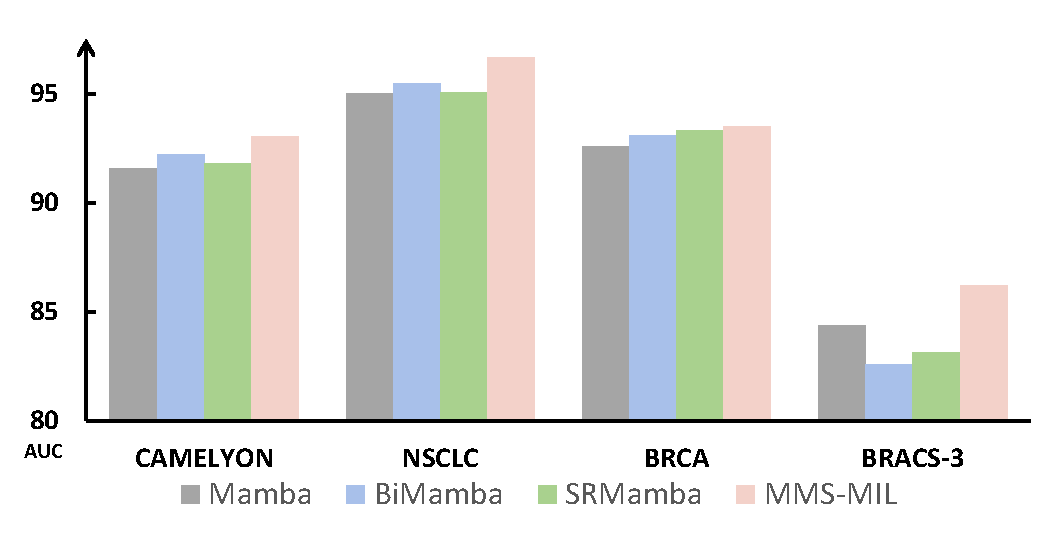
\includegraphics[width=0.9\columnwidth]{figures/MMSMIL的不同Mamba比较.pdf}
  \bicaption[不同Mamba模型的性能比对柱状图]{不同Mamba模型的性能比对柱状图。}[Bar chart of performance comparison of different Mamba models.]{Bar chart of performance comparison of different Mamba models.}
  \label{figure3: DifferentMamba}
  % \vspace{-4pt}
\end{figure}
\textbf{(2)不同Mamba模型性能比对}



为了进一步验证本章的方法的优越性来源于本章的架构而不是Mamba本身,本章对三种变体进行了比较实验:图\ref{figure3: DifferentMamba}中的Mamba Block、BiMamba和SRMamba。
结果表明,M$^2$S-MIL在所有四个数据集上都取得了最佳性能。
本章的方法不仅在性能上超过了原始的单分支Mamba,而且在与没有引入局部连续性和旋转不变性等视觉图像的聚合方法(例如,BiMamba和SRMamba)的比较中表现出许多优势。
实验结果表明,本章的引入2D特性的Mamba比其他多扫描综合的Mamba算法具有更强的实例建模能力,更强的空间信息捕获能力,能够提取更多的判别性特征。



\textbf{(3)讨论区域数量对模型性能的影响}

\begin{figure}[ht]
  \centering
  \captionsetup{font={small, stretch=1.312}}
  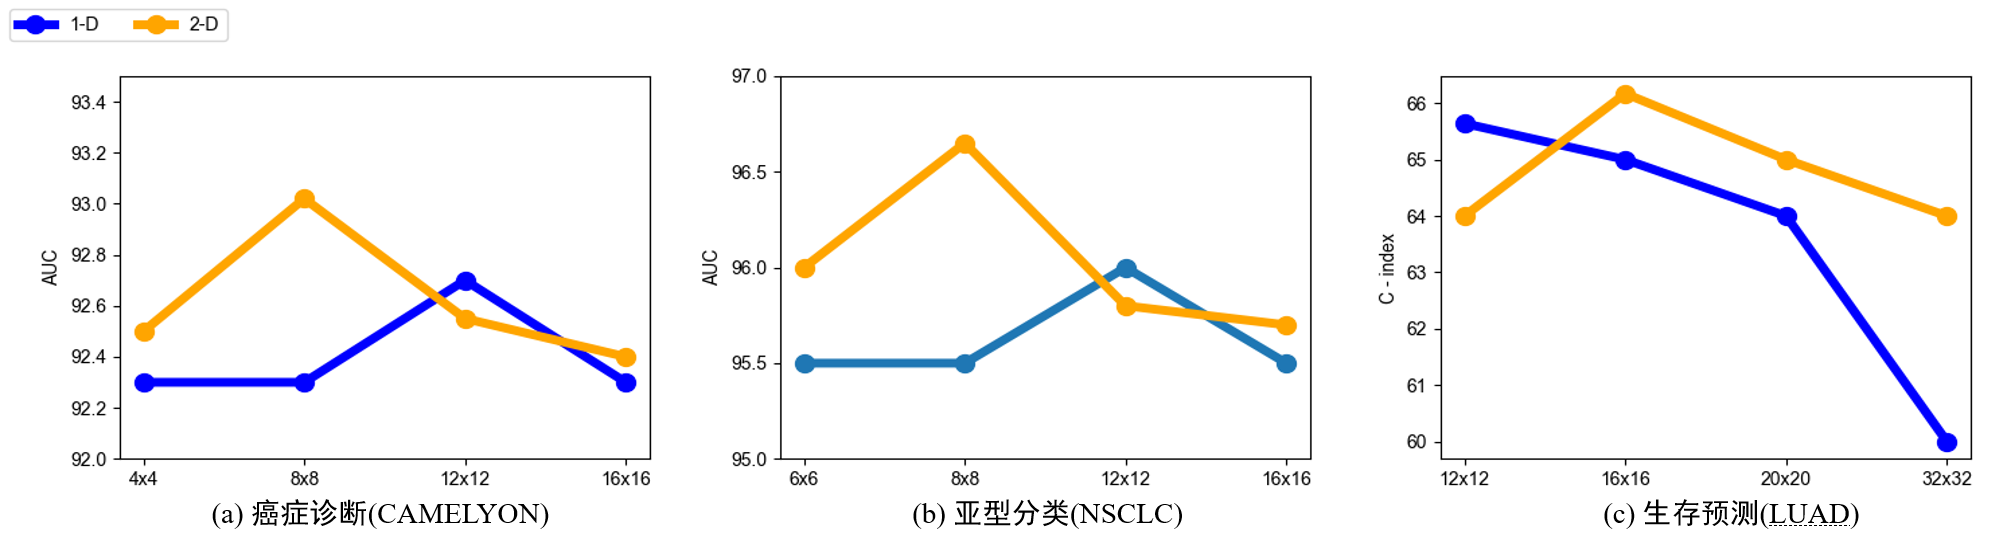
\includegraphics[width=1.0\columnwidth]{figures/区域个数.png}
  \bicaption[不同区域数量的模型性能折线图]{不同区域数量的模型性能折线图。}[Breakpoint plots of model performance for different number of regions]{Breakpoint plots of model performance for different number of regions.}
  \label{figure3: NumOfRegion}
\end{figure}

本小节系统地研究了不同区域划分策略在本章的方法中的影响。图~\ref{figure3: NumOfRegion}展示了不同区域划分在病理分类任务上的性能效果,其中1-D代表并不将之重塑为2D特征图而只进行一维序列的分区。
从与1D的对比实验可以看出,二维区域划分方式优于一维区域划分方式,因为它保留了更多的原始图像的空间信息。
并且本章认为,本章的性能提升并不仅仅依赖于对序列简单的划分区域,侧面印证了本章方法,通过引入更多空间信息从而提高了模型性能。
此外,另一个现象是,使用过小或过大的区域会使性能下降。这是因为小区域大幅降低了Mamba建模二维关系的能力(近似正常原始序列输入),而过大的区域将原本相距较远不具备连续性的特征关联在一起导致性能损耗。
因此,采用适中的区域划分是多扫描Mamba输入的最佳选择。


\textbf{(4)窗口大小对2D 空间上下文感知模块的影响分析}

\begin{table}[h!]
  \large    % 设置表格字体为5号
  \setstretch{1.245}        % 设置具有指定弹力的橡皮长度(原行宽的1.2倍)
  \captionsetup{font={small, stretch=1.512}}
  \centering
  % \vspace{-10pt}
  \bicaption[不同大小窗口对性能影响]{不同大小窗口对性能影响。最优结果用粗体表示。}{Effect of different window sizes on performance. The best results are shown in bold.}    % 中英文标题
  \begin{tabularx}{\textwidth}{lCCCC}
    \toprule
    方法 & CAMELYON& NSCLC&BRCA&BRACS3\\ \midrule
    W/o  & 92.72$\pm$1.82 &  96.25$\pm$1.44 & 93.01$\pm$1.82 &  85.24$\pm$0.32\\
    3 $\times$ 3  &  92.78$\pm$1.52 & 96.31$\pm$1.33 & 93.37$\pm$1.93 & 85.71$\pm$1.80\\
  \textbf{5 $\times$ 5} &\textbf{93.02$\pm$1.20} &\textbf{96.65$\pm$1.08}  &\textbf{93.50$\pm$1.70} & \textbf{86.21$\pm$0.46}\\
    \bottomrule
  \end{tabularx}
  % \vspace{-25pt}
  \label{table3: size of window}
\end{table}

本小节探究了不同窗口大小的2D空间上下文感知模块对M$^2$S-MIL的性能影响。
可以看到越大窗口范围可以整合更多的空间信息,所带来的性能提升越大。
但是由于计算窗口注意力所需要的计算资源随窗口大小增大而增大,所以平衡计算资源与性能之间选择适中的窗口大小是M$^2$S-MIL的最佳选择。

\textbf{(5)使用PLIP作为特征提取器的性能结果}

\begin{table}[h!]
  \large    % 设置表格字体为5号
  \setstretch{1.245}        % 设置具有指定弹力的橡皮长度(原行宽的1.2倍)
  \captionsetup{font={small, stretch=1.512}}
  \centering
  % \vspace{-10pt}
  \bicaption[M$^2$S-MIL以PLIP为离线特征提取器的亚型分型性能]{M$^2$S-MIL以PLIP为离线特征提取器的癌症诊断性能。最优结果用粗体表示,次优结果用下划线表示。}{Cancer diagnosis performance of M$^2$S-MIL with PLIP as the offline feature extractors. The optimal experimental results are marked in bold, and the sub-optimal are underlined.}    % 中英文标题
  \begin{tabularx}{\textwidth}{clCCC}
    \toprule
    &方法  & Accuracy& AUC&F1 - score\\ \midrule
    \multirow{5}{*}{\rotatebox{90}{PLIP}}&AB - MIL  & 90.09$\pm$1.63 & \underline{94.55$\pm$1.91} & 86.48$\pm$2.50\\
    &OriginMamba        & 90.87$\pm$1.52 & 94.44$\pm$2.19 & 87.78$\pm$1.89\\
    &BiMamba          & 90.54$\pm$1.89 & 94.20$\pm$1.99 & 86.82$\pm$2.77\\
    &SRMamba & \underline{91.87$\pm$0.85} & 94.20$\pm$2.16 & \underline{88.37$\pm$1.31}\\
    &\textbf{M$^2$S - MIL}        & \textbf{92.21$\pm$0.60}     & \textbf{95.24$\pm$1.85}      & \textbf{89.46$\pm$0.93}\\  
    \bottomrule
  \end{tabularx}
  % \vspace{-25pt}
  \label{table3: CAMELYON_PLIP}
\end{table}

\begin{table}[h!]
  \large    % 设置表格字体为5号
  \setstretch{1.245}        % 设置具有指定弹力的橡皮长度(原行宽的1.2倍)
  \captionsetup{font={small, stretch=1.512}}
  \centering
  % \vspace{-10pt}
  \bicaption[M$^2$S-MIL以PLIP为离线特征提取器在TCGA-NSCLC上的亚型分型性能]{M$^2$S-MIL以PLIP为离线特征提取器在TCGA-NSCLC上的亚型分型性能。最优结果用粗体表示,次优结果用下划线表示。}{Cancer sub-typing performance of M$^2$S-MIL on the TCGA-NSCLC dataset with PLIP as the offline feature extractors. The optimal experimental results are marked in bold, and the sub-optimal experimental results are underlined.}    % 中英文标题
  \begin{tabularx}{\textwidth}{clCCC}
    \toprule
    &方法  & Accuracy& AUC&F1 - score\\ \midrule
    \multirow{5}{*}{\rotatebox{90}{PLIP}}&AB - MIL  & 89.94$\pm$1.84 & 94.45$\pm$1.64 & 89.43$\pm$1.97\\
    &OriginMamba        & \underline{90.89$\pm$1.60} & 95.57$\pm$1.60 & \underline{90.24$\pm$1.84}\\
    &BiMamba          & 90.70$\pm$1.95 & 95.42$\pm$1.68 & 89.94$\pm$2.26\\
    &SRMamba &  89.85$\pm$2.07 &  \underline{95.72$\pm$1.51} & 88.96$\pm$2.66 \\
    &\textbf{M$^2$S - MIL}        & \textbf{91.56$\pm$1.76}     & \textbf{96.22$\pm$1.12}      & \textbf{90.64$\pm$1.86}\\   
    \bottomrule
\end{tabularx}

  \label{table3: NSCLC_PLIP}
\end{table}


\begin{table}[h!]
  \large    % 设置表格字体为5号
  \setstretch{1.245}        % 设置具有指定弹力的橡皮长度(原行宽的1.2倍)
  \captionsetup{font={small, stretch=1.512}}
  \centering
  % \vspace{-10pt}
  \bicaption[M$^2$S-MIL以PLIP为离线特征提取器在TCGA-BRCA上的亚型分型性能]{M$^2$S-MIL以PLIP为离线特征提取器在TCGA-BRCA上的亚型分型性能。最优结果用粗体表示,次优结果用下划线表示。}{Cancer sub-typing performance of M$^2$S-MIL on the TCGA-BRCA dataset with PLIP as the offline feature extractors. The optimal experimental results are marked in bold, and the sub-optimal experimental results are underlined.}    % 中英文标题
  \begin{tabularx}{\textwidth}{clCCC}
    \toprule
    &方法  & Accuracy& AUC&F1-score\\ \midrule
    
  \multirow{5}{*}{\rotatebox{90}{PLIP}}&AB-MIL  & 83.81$\pm$3.72 & 90.18$\pm$2.99 & 67.94$\pm$4.22\\
  &OriginMamba        & 86.75$\pm$5.76 & \underline{92.90$\pm$2.44} & \underline{74.35$\pm$7.23}\\
  &BiMamba          & \underline{87.73$\pm$3.06} & 92.64$\pm$2.28 & 74.07$\pm$4.75\\
  &SRMamba & 86.40$\pm$3.31 & 92.17$\pm$2.67 & 72.39$\pm$4.62\\
  &\textbf{M$^2$S-MIL}        & \textbf{88.82$\pm$3.22}     & \textbf{93.40$\pm$1.24}      & \textbf{75.00$\pm$2.50}\\  
  \bottomrule
\end{tabularx}
  \label{table3: BRCA_PLIP}
\end{table}





为了进一步探索本章方法的有效性,本小节还进行了将同样采用自监督预训练的PLIP~\cite{huang2023visual}作为特征提取器的相关实验,以验证本章方法的普遍性。
如表\ref{table3: CAMELYON_PLIP}、\ref{table3: NSCLC_PLIP}和表\ref{table3: BRCA_PLIP}所示,可以看出实验结果与R50特征一致。
本章的方法优于其他基于Mamba的方法。在CAMELYON数据集上,它在Accuracy、AUC和F1-score方面分别比次优的方法提高了0.34\%、0.69\%和1.09\%。这些数据在NSCLC数据集中分别为0.57\%,0.4\%和0.4\%。
最后,BRCA数据集的改进也值得注意,Accuracy提高了1.09\%,AUC提高了0.5\%,F1-score提高了0.65\%。
这进一步表明,即使使用非传统的ResNet-50特征提取器,本章方法的性能改进也不仅仅是依赖于简单的多个Mamba分支合并,而是正确捕获了空间信息与视觉特征。


\begin{figure}[ht]
  \centering
  \captionsetup{font={small, stretch=1.312}}
  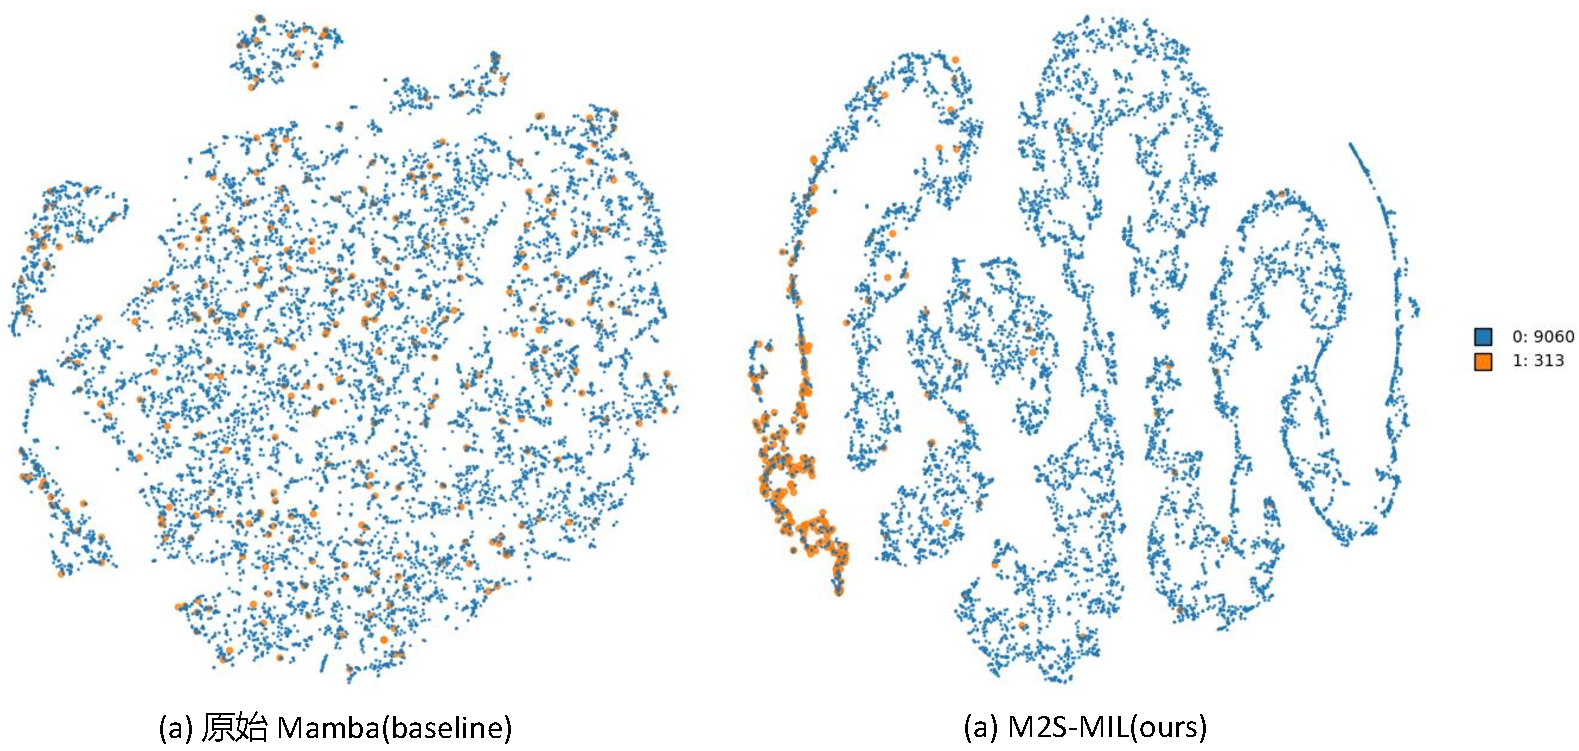
\includegraphics[width=1.0\columnwidth]{figures/vis2_2.pdf}
  \bicaption[原始Mamba(baseline)和M$^2$S-MILL聚合特征t-SNE可视化结果]{原始Mamba(baseline)和M$^2$S-MIL聚合特征t-SNE可视化结果。}[The t-SNE visualization of aggregated features from original Mamba(baseline) and SMC-MIL]{The t-SNE visualization of aggregated features from Mamba(baseline) and SMC-MIL.}
  \label{figure3: tSNE}
\end{figure}

\subsection[\hspace{-2pt}可视化分析]{{\heiti\zihao{4} \hspace{-8pt}可视化分析}}\label{section3: 可视化分析}
\begin{figure}[h!]
  \centering
  \captionsetup{font={small, stretch=1.312}}
  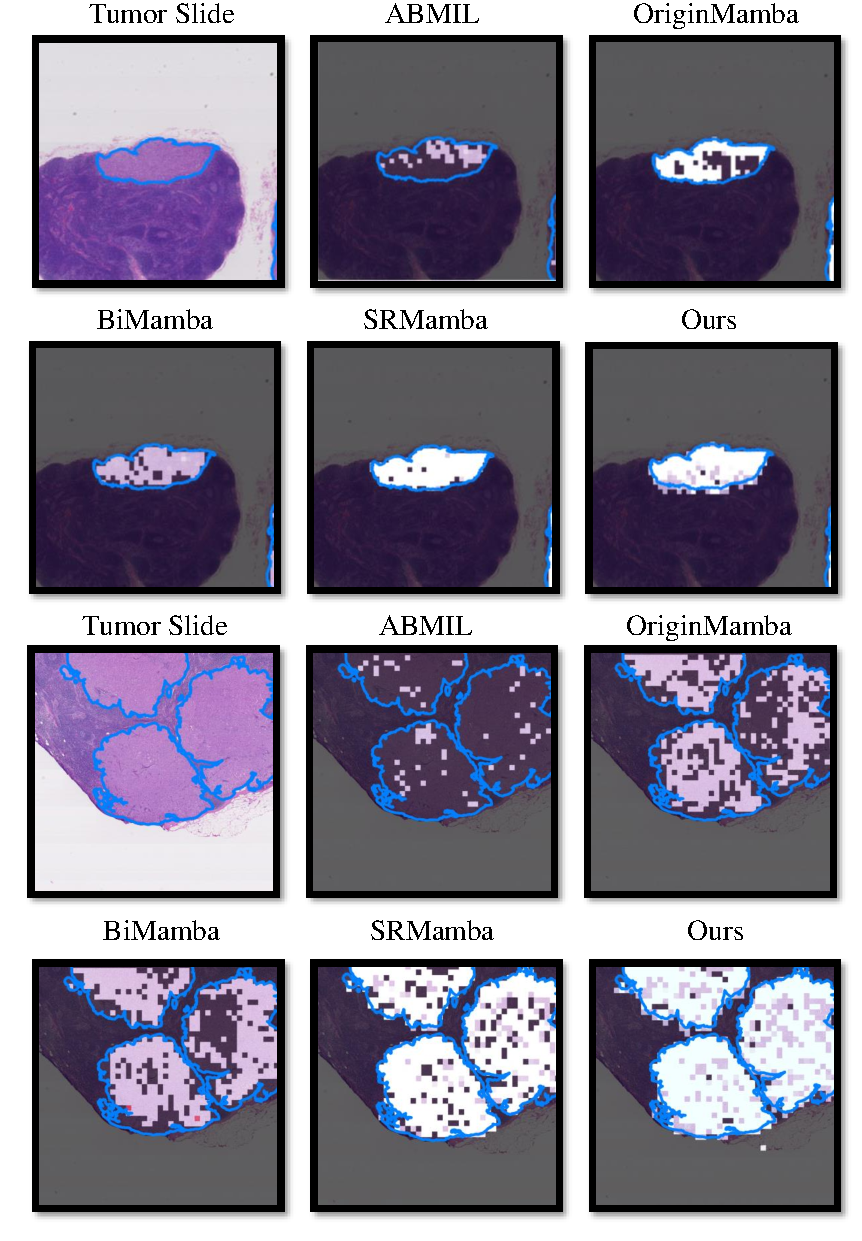
\includegraphics[width=0.7\columnwidth]{figures/vis2.pdf}
  \bicaption[多个Mamba变体和M$^2$S-MIL关注的图块可视化结果]{多个Mamba变体和M$^2$S-MIL关注的图块可视化结果}[Visualization results of patches focused by other Mamba and SMC-MIL]{Visualization results of patches focused by other Mamba variants(baseline) and SMC-MIL.}
  \label{figure3: visualize}
\end{figure}

为了直观地验证本章方法的可解释性,本章用t-SNE可视化了同一个WSI切片的所有实例经过Mamba和M$^2$S-MIL所建模出后的特征,结果展示在图\ref{figure3: tSNE}。
可以看到M$^2$S-MIL更具有条理,而原始Mamba的结果更为混乱。说明M$^2$S-MIL使Mamba的实例间的关系建模能力更为出色。

并且本章将多种Mamba变体与本章的方法在Camelyon-16数据集上产生的高注意力分数的实例可视化,如图\ref{figure3: visualize}所示。
蓝色的线条勾勒出肿瘤区域。越亮的斑块表明注意力得分越高。
可视化结果清楚地表明,与原始Mamba相比,M$^2$S-MIL能够更准确地选择显著斑块。
 

\section[\hspace{-2pt}本章小结]{{\heiti\zihao{-3} \hspace{-8pt}本章小结}}\label{section3: 本章小结}

本章针对序列关系建模模型Mamba在处理数字病理图像分类任务时,对视觉任务特性和空间关系捕捉不充分的问题,
提出了一种简单有效的解决思路,并提出一种新的多实例学习方法:
基于空间信息增强的多扫描Mamba的数字病理图像分类(Multi-scan Mamba with Sptial information enhancement,简称M$^2$S-MIL)。
该方法通过综合多种扫描模式的信息,针对病理图像空间信息,设计了区域螺旋扫描和网格扫描模式,增强Mamba对病理图像空间关系的建模。
同时利用2D空间上下文感知模块,进一步对整合后的序列进行空间关系增强,提升模型性能。
在3个WSI子任务以及7个数据集上的大量对比及消融实验充分证明了,本章提出的基于空间信息增强的多扫描Mamba的多实例学习架构综合了多种扫描模式分支,
引入空间信息,解决了数字病理图像分类任务中使用Mamba模型存在的图像空间结构捕获能力不足的问题。
%未来,作者将计划进一步探索如何在更有限的扫描模式序列情况下,使Mamba更高效更好地捕获空间关系,更充分建模实例间关系。